\section{Use Cases and Sequence Diagrams}
\label{sec:use-cases}

% ---------- Use Case 1: D'Artagnan Passailaigue ----------

\subsection{Use Case 1: Executing a Command in a Local Pane}

\label{sec:use-case-1}

In this local-pane use case, the Mux Server lifeline represents the local session-management role. Figure 1 shows the same role deployed on the remote host for SSH multiplexing.

The sequence diagram illustrated below demonstrates the control and data flow that occurs when a user opens a local pane in WezTerm and executes a command. The interaction begins when the User opens a local pane through the GUI Front End. The GUI Front End communicates with the Multiplexer, which creates or accesses the appropriate local Mux Server and establishes a connection to the PTY. The PTY provides the interface between the terminal environment and the Shell, which is responsible for interpreting and executing commands.

Once the local pane has been established, the User enters the \texttt{ls} command. The GUI Front End receives this keyboard input and passes it through the Multiplexer and local Mux Server to the PTY, which forwards the input to the Shell. The Shell interprets the command and requests that the operating system perform the corresponding operation. The resulting output is returned through the Shell and PTY to the local Mux Server. The output is then passed through the Multiplexer to the Terminal Emulation Core, which processes the terminal data and updates the terminal state. Finally, the processed output is sent to the GUI Front End, which renders the result in the local terminal pane for the User to see.

The activation boxes on each lifeline represent the periods during which each component is actively processing the request. Overall, the diagram illustrates both control flow, as each component triggers the next stage of processing, and data flow, as the user's command and the resulting output move through the GUI Front End, Multiplexer, local Mux Server, PTY, Shell, and Terminal Emulation Core before being displayed to the User. This is one example of how local panes may be used in WezTerm, but it was selected for this example because of its straightforward execution and general simplicity.

\subsubsection{Sequence Diagram: Executing a Command in a Local Pane}

\label{sec:local-command}

\begin{figure}[H]
    \centering
    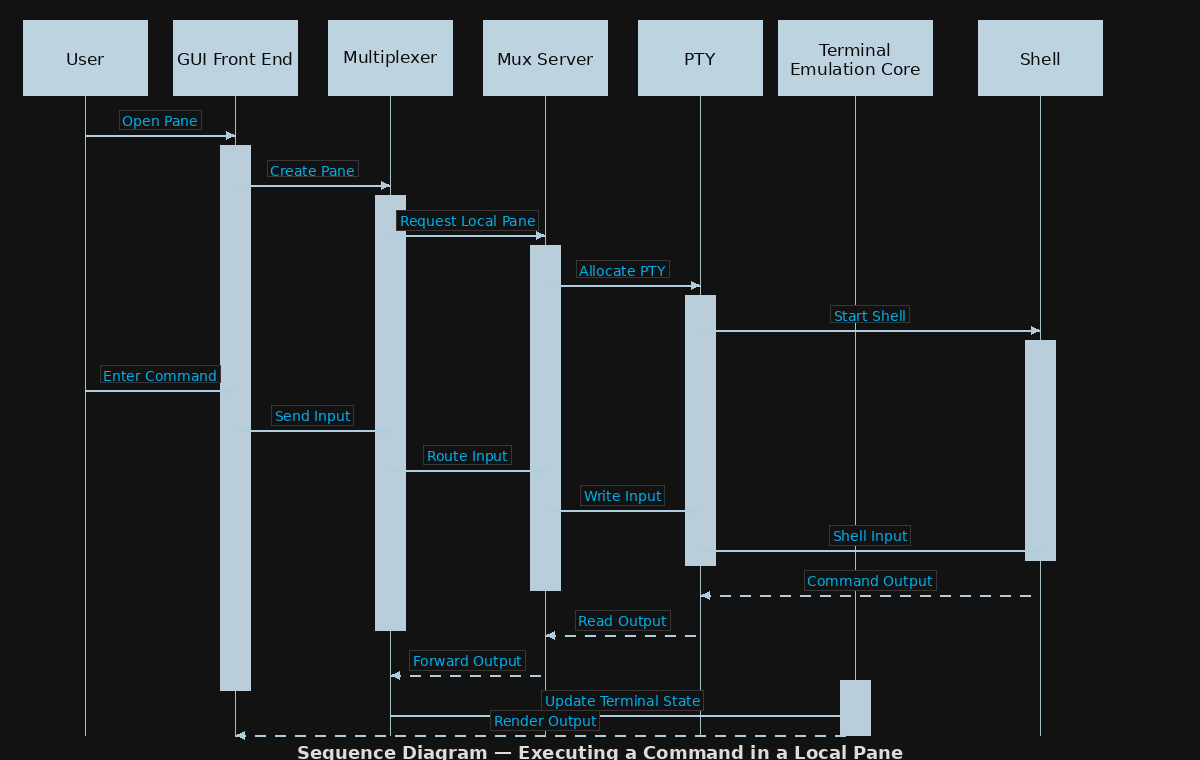
\includegraphics[width=0.7\linewidth]{figures/local_pane_architecture_sequence_diagram(1).png}
    \caption{Sequence diagram: executing a command in a local pane.}
    \label{fig:use-case-1}
    \caption*{Legend: boxes and lifelines represent participants; solid arrows are messages, dashed arrows are replies, and activation bars show active processing.}
\end{figure}

The Sequence Diagram shown in Figure~\ref{fig:use-case-1} describes the interaction between components as the user executes a command in a local pane. The diagram follows the command from the User through the GUI Front End, Multiplexer, local Mux Server, PTY, and Shell, before tracing the resulting output back through the Terminal Emulation Core and GUI Front End.

\FloatBarrier
% ---------- Use Case 2: Jeremy McCrindle ----------
% Diagrams are TikZ, generated from ssh-mux/ (run ssh-mux/export_latex.sh after editing them).
% If a TikZ figure gives trouble, swap \diagram{<name>.tex} for its PNG backup:
% \includegraphics[width=\linewidth]{<name>.png}
\subsection{Use Case 2: Remote Work over SSH}
\label{sec:use-case-2}

In this example, we follow a user who already has WezTerm open with several local tabs running. The user works on a remote host whose panes are kept by a Mux Server, ensuring persistence on a session drop \cite{multiplexing}. We trace how control and data flow between WezTerm's components in three stages: the user attaches to a remote build machine (devbox) through an SSH multiplexing domain, the user sends commands in a remote tab, and the user ends the remote session. As the first and last stages are the start and end of the same session, they share one sequence diagram.

\subsubsection{Sequence Diagram: Attaching to and Detaching from a Remote Host}
\label{sec:ssh-lifecycle}

The Sequence Diagram shown in Figure~\ref{fig:ssh-lifecycle} describes the user attaching to a remote SSH server and later ending the session. It begins with the user selecting an SSHMUX domain from WezTerm's launcher menu, which issues an attach request for that domain \cite{multiplexing}. The connection is then set up in six steps:

\begin{figure}[!tbp]
  \centering
  \diagram{ssh-mux-seq13-lifecycle.tex}
  \caption{Sequence diagram: attaching to and detaching from a remote host.}
  \label{fig:ssh-lifecycle}
\end{figure}

\begin{enumerate}
  \item The GUI Front End passes the request asynchronously to the Multiplexer.
  \item The Multiplexer requests that the Mux Client attach to the selected domain.
  \item The Mux Client asks the SSH Client to open a session with the remote host. If the host key is unknown or a passphrase is needed, a prompt appears in the GUI Front End awaiting the user's response.
  \item The SSH Client then runs a WezTerm proxy on the remote host, which starts the Mux Server if none is running and connects to it. From this point on, the SSH connection only carries messages between the Mux Client and the Mux Server.
  \item The Mux Client checks that both ends use a compatible protocol version, then fetches the remote host's windows, tabs and panes.
  \item The remote panes are added to the Multiplexer alongside the local ones, and the Multiplexer notifies the GUI Front End, which displays the new tab.
\end{enumerate}

Importantly, the user's local tabs continue to run as normal while attaching to a remote host, as demonstrated by the par fragment in Figure~\ref{fig:ssh-lifecycle}. Once the domain is attached, any new tab the user opens from a remote pane is created on the remote server by default, so the user stays on the remote host until they explicitly switch back.

A remote session can end in three ways, though only the first two are shown in the diagram, as operands of the alt fragment. In all three cases, the user's local tabs remain unaffected.

\begin{itemize}
  \item A user detach from the SSH multiplexing domain occurs after the user manually detaches from the pane or closes the window. The panes keep running on the Mux Server, so the user is able to reattach and find them in the same state.
  \item A network disconnect from the remote host occurs after the SSH Client reports a read error or timeout and the Mux Client drops the domain's panes locally. WezTerm does not reconnect SSH domains automatically, but the panes keep running on the Mux Server, so the user is able to reattach.
  \item A program exit from a remote pane occurs after the program running in it ends. Only that pane closes, along with its tab if it was the last pane in it, while the Mux Server keeps running.
\end{itemize}

Since the documentation does not cover network loss in detail, its flow in Figure~\ref{fig:ssh-lifecycle} is our interpretation of WezTerm's changelog and a developer comment in its source code \cite{client-source}.


\clearpage

\subsubsection{Sequence Diagram: Sending Keyboard Input to a Remote Pane}
\label{sec:ssh-input}

The Sequence Diagram shown in Figure~\ref{fig:ssh-input} describes the interaction between components as the user sends keyboard input in a remote tab, following a single key press to the remote shell and back. In transit, the key press passes from the GUI Front End to the Multiplexer, which hands it to the Mux Client as the pane belongs to a remote server. The Mux Client then sends the key press to the Mux Server asynchronously. The Mux Server writes it to the remote PTY, where the shell, an external program, processes the input. The shell's output then travels back to the GUI Front End in three steps:

\begin{enumerate}
  \item A reader thread on the remote host passes the output to the Terminal Emulation Core, which interprets it and updates the pane's screen.
  \item The Mux Server sends the lines of the screen that changed to the Mux Client.
  \item The Multiplexer notifies the GUI Front End that the pane has new output, and the GUI Front End redraws it.
\end{enumerate}

\begin{figure}[!htbp]
  \centering
  \scalebox{0.85}{\diagram{ssh-mux-seq2-dataflow.tex}}
  \caption{Sequence diagram: sending keyboard input to a remote pane.}
  \label{fig:ssh-input}
\end{figure}

An inherent drawback is that every key press has to travel across the network and back before it appears on screen. To hide this delay on slow connections, the Mux Client predicts how the typed character will appear and shows it immediately once the delay passes a set threshold, then replaces the prediction when the real output arrives \cite{sshdomain}.